\documentclass[11pt,a4paper]{article}
\usepackage{fontspec}
\setmainfont{TeX Gyre Pagella}
\newfontfamily\headfont{Inter}[UprightFont=*-ExtraBold,BoldFont=*-ExtraBold,Extension=.otf,Path=/usr/share/fonts/opentype/inter/]
\usepackage[a4paper,margin=2.4cm]{geometry}
\usepackage{graphicx,booktabs,float,caption,array,xcolor,longtable,amsmath}
\usepackage{xurl}
\usepackage[hidelinks]{hyperref}
\usepackage{titlesec}
\usepackage[round,sort]{natbib}
\usepackage{setspace}
\setstretch{1.12}
\renewcommand{\topfraction}{0.9}
\renewcommand{\bottomfraction}{0.8}
\renewcommand{\textfraction}{0.1}
\renewcommand{\floatpagefraction}{0.75}
\setlength{\parindent}{1.2em}
\setlength{\parskip}{0.25em}
\titleformat{\section}{\headfont\Large}{\thesection}{0.8em}{}
\titleformat{\subsection}{\headfont\large}{\thesubsection}{0.8em}{}
\captionsetup{font=small,labelfont=bf}
\urlstyle{same}
\providecommand{\doi}[1]{\url{https://doi.org/#1}}
\hypersetup{pdftitle={Roundhead or Cavalier, Leave or Remain?},pdfauthor={Tristan Hotham}}

\begin{document}
\begin{center}
{\Large\bfseries Roundhead or Cavalier, Leave or Remain?\par}
\vspace{0.4em}
{\large The Danelaw, Civil War allegiance and the 2016 referendum in England and Wales\par}
\vspace{1.2em}
{\large Dr Tristan Hotham\par}
\vspace{0.3em}
{\small Independent researcher\\
ORCID: 0000-0003-4931-9349\\
Data and code: https://doi.org/10.5281/zenodo.24104516\par}
\vspace{0.8em}
2026
\end{center}

\begin{quote}
\small
\begin{center}\textbf{Abstract}\end{center}
Maps that set the 2016 Leave vote beside very old divisions of England are widely shared, and a large literature asks whether historical shocks leave lasting political traces. I test two such divisions against Hanretty's estimated Leave share in 2010 Westminster constituencies, following an analysis plan written before any outcome model was run. The first is the Danelaw, drawn from the boundary clause of the treaty of Alfred and Guthrum and the conventional line along Watling Street to Chester. Seats on the Danelaw side voted Leave by 6.9 points more on average, but with region fixed effects and controls for density and 2011 census composition the difference is -0.16 points (95\% CI -1.81 to 1.49; N = 533). A boundary design along the line gives estimates that change sign with the bandwidth and a jump at a placebo line, while Scandinavian place-name endings do jump at the line. The second is Civil War allegiance, coded from the Long Parliament: 201 of the 507 seats returned in 1640 had members who later sided with the King. A county's royalist share has a small negative conditional association with Leave, -0.30 points per 10 points of royalist share (95\% CI -0.56 to -0.05; N = 558), but the wild cluster bootstrap p-value is 0.07 and the estimate is not robust to several planned checks. Neither old line adds much to what the present composition of places already explains. The design is cross-sectional and correlational.

\textbf{Keywords:} Brexit; Danelaw; English Civil War; historical persistence; electoral geography; boundary design; England and Wales
\end{quote}

\section{Introduction}\label{sec:intro}
Since the 2016 referendum on membership of the European Union, maps of the result have often been set beside maps of much older divisions of England. The pairings were striking. The east of England, much of which voted to leave, looked a little like the Danelaw, the area under Scandinavian rule and law after the wars of the ninth century; the counties that held for Parliament against Charles I in the 1640s, around London and the south-east, looked a little like the places where Remain was strongest. These comparisons are not idle. They express a popular theory of politics in which places carry long memories, and a scholarly literature has shown that historical events can shape political behaviour for generations \citep{satyanath2017,rodden2019}. They also carry a risk familiar to anyone who has compared two maps: places close to each other are alike in many ways, and two maps of anything that varies smoothly across England will tend to resemble each other.

This paper puts two of these comparisons to a planned test. The question is not whether the Danelaw or the Civil War caused anything in 2016; with a single cross-section that cannot be shown. It is the narrower question of whether either old division predicts the estimated Leave share of a constituency once the obvious present-day differences between places are held fixed: region, population density, distance to a city, and the age, education, class, ethnicity, birthplace, housing, industry and health of the people who live there now. If an old line still marks something about political attitudes that today's composition does not, it should show up here. If it does not, the resemblance of the maps is more likely to be a resemblance of places than a persistence of history.

The contribution is threefold. First, I construct two historical exposures at the level of the 2010 constituency in England and Wales. The Danelaw is measured three ways: by a line drawn from the boundary clause of the treaty of Alfred and Guthrum and the conventional continuation along Watling Street \citep{davis1982,dumville1992}, by the fifteen shires assigned to Danish law in the medieval shire lists \citep{downer1972,wikithreefold}, and by the share of each seat's settlements whose names carry Scandinavian endings. Civil War allegiance is measured from people rather than territory: for each historic county, the share of the members returned to the Long Parliament in 1640 who were later disabled from sitting for siding with the King, coded from the notes of the list of members \citep{wiki1640} with every hand decision documented. Second, I test both exposures against the Leave vote with a plan written before any outcome model was run, with a model ladder, a boundary design, placebo lines, permutation and wild cluster bootstrap inference, and leave-one-out checks. Third, I report the results plainly. The Danelaw gap of 6.9 points in the raw data disappears once like is compared with like (-0.16 points), and the boundary design is too unstable to support any claim. The Civil War measure has a small negative conditional association with Leave, the opposite of the ``Cavalier counties voted Leave'' reading of the maps, but it is not robust.

Section~\ref{sec:lit} reviews the literature on the geography of the Leave vote, on historical persistence, and on the two divisions. Section~\ref{sec:data} describes the data and the construction of the exposures, Section~\ref{sec:design} the plan and the models, Section~\ref{sec:results} the results and Section~\ref{sec:robust} the robustness checks. Section~\ref{sec:disc} discusses what the results do and do not show.

\section{Background and literature}\label{sec:lit}
\subsection{The geography of the Leave vote}
The geography of the referendum is one of the best-studied facts in recent British politics. Estimated at the level of local authorities and, by areal interpolation, Westminster constituencies \citep{hanretty2017}, the Leave share was highest in older, whiter and less educated places, in places with more manufacturing and less in-migration from abroad, and lowest in London, the university cities and Scotland \citep{becker2017,goodwin2016,harris2016,alabrese2019}. Education and age carry most of the explanatory weight in district-level models; \citet{becker2017} find that a small set of fundamental characteristics accounts for most of the variation across districts. Economic shocks add to the picture: import competition from China \citep{colantone2018}, austerity \citep{fetzer2019} and long-term economic distress \citep{carreras2019} are each associated with more Leave voting. A related literature casts the vote as a revolt of places left behind, whose long-run decline was turned into a political force \citep{rodriguezpose2018,mccann2020,dijkstra2020,lee2018}, and others stress the cultural and social context of places \citep{abreu2020,jennings2016,furlong2019,johnston2018}. Studies of individual voters reach compatible conclusions about age, education and attitudes \citep{hobolt2016,clarke2017}, and the long build-up of support for UKIP before the referendum followed the same lines \citep{ford2014}.

Two features of this literature matter here. First, a small set of present-day characteristics explains most of the variation in the Leave vote across places. Any historical exposure that is correlated with those characteristics will appear to predict Leave in a raw comparison. Second, the composition of places today is itself partly a product of history. Controlling for it asks whether an old division adds anything beyond the places it helped to make, and that is the question asked here; the total association, including any path that runs through composition, is reported as well but cannot be separated from confounding with these data.

\subsection{Historical persistence}
A large literature in economics and political science asks whether historical events and institutions leave traces in present-day behaviour. Among the best-known designs are those that relate a historical feature of places to a modern outcome while holding modern conditions fixed; \citet{satyanath2017}, for example, relate the density of civic associations in German towns before 1933 to entry into the Nazi Party, \citet{voigtlaender2012} find that towns with pogroms during the Black Death in 1348 to 1350 showed more violence against Jews in the 1920s and higher Nazi Party votes, \citet{fouka2023} show that memories of German reprisals in Greece during the Second World War resurfaced in the debt crisis of 2009 and reduced purchases of German cars most in the places that had suffered them, and \citet{rodden2019} traces the urban-rural divide in American voting to the location of nineteenth-century industry. \citet{alesina2015} review the wider evidence that culture and institutions shape each other over long periods. Two lessons from this literature shape the design here. The first is that historical exposures are rarely assigned at random, so their association with an outcome can reflect the geography of the places they cover rather than the history itself. The second is that spatial data have spatially correlated errors, which can make associations look more precise than they are; standard responses are clustering at a level that captures the dependence, spatial standard errors \citep{conley1999}, and randomisation-based tests. Because boundaries can create sharp contrasts between otherwise similar places, boundary designs that compare places just either side of an old line are also common; \citet{keele2015} show that such a geographic boundary design is a regression discontinuity with two running variables, and that its validity rests on the absence of other jumps at the line, which can be checked with pre-treatment covariates.

The present study applies these tools to two historical divisions that are frequently invoked in public discussion of the referendum. It is a test of a popular claim rather than of a theory with a specific mechanism. That has a cost, since without a mechanism there is no strong prior about the sign, and a benefit, since a planned test of a widely repeated claim is useful whatever it finds.

\subsection{The Danelaw}
The treaty of Alfred and Guthrum, usually dated to the 880s, sets out a boundary between the English and the Danish-ruled territory: up the Thames, up the Lea to its source, then straight to Bedford, then up the Ouse to Watling Street \citep{dumville1992}. The course and the date of the frontier have been discussed at length \citep{davis1982,dumville1992,hart1992}. Beyond Watling Street the treaty is silent, and the conventional maps continue the line north-west along the Roman road. The western bounds may have lasted no more than seven years \citep{rochester2023}, and the reconquest of the Danish-held territory by the kings of Wessex began within a generation. The name ``Danelaw'' itself belongs to the later legal history of England, in which the law of the Danes was one of three bodies of law alongside those of Wessex and Mercia \citep{downer1972,wormald1999,abrams2008}. Medieval shire lists assign fifteen shires to Danish law: Yorkshire, Nottinghamshire, Derbyshire, Leicestershire, Lincolnshire, Northamptonshire, Huntingdonshire, Cambridgeshire, Bedfordshire, Norfolk, Suffolk, Essex, Hertfordshire, Middlesex and Buckinghamshire \citep{wikithreefold}. This legal Danelaw is not the same area as the treaty line: it includes Buckinghamshire and Middlesex, which lie partly or wholly on the English side of the treaty line, and leaves out the far north.

The most durable trace of Scandinavian settlement in England is in its place-names. Names ending in \emph{-by}, \emph{-thorpe}, \emph{-thwaite} and \emph{-toft} are concentrated in the north and east \citep{watts2004,gelling2000}, though thorp names have mixed Old English and Old Norse origins \citep{cullen2011} and Scandinavian names also occur beyond the treaty line \citep{fellowsjensen2014}. Archaeological finds of Scandinavian-style metalwork show a similar eastern concentration \citep{kershaw2013}. The genetic trace is faint: a fine-scale study of the British population found no clear genetic evidence of the Danish Viking occupation of a large part of England, suggesting a relatively limited input \citep{leslie2015}. The Danelaw, then, is a real division in the historical record, but a fuzzy one: the line was short-lived, its north-western course is conventional, the legal Danelaw differs from the treaty area, and the intensity of Scandinavian settlement varied greatly within it. I use all three measures for that reason.

\subsection{The Civil War}
The First Civil War (1642 to 1646) divided the political nation. The House of Commons elected in 1640, the Long Parliament, split as war approached: members who joined the King were ``disabled'' from sitting, and many sat in the King's assembly at Oxford. The social and regional composition of the two sides was studied in detail by \citet{brunton1954}, whose work was central to the debate about the social interpretation of the English Revolution \citep{zagorin1959}. Allegiance had a strong regional pattern: Wales, the west and the north provided much of the King's support among members, while London, the south-east and East Anglia were Parliament's heartland. In Wales, seventeen of the twenty-four members joined the King \citep{dodd1952,zagorin1959}. Territorial control is a different matter from members' allegiance: it shifted with the campaigns, and contemporary-style maps of the districts held by each side at given dates exist in historical atlases \citep{gardiner1914}. Here I measure allegiance through members, which can be coded systematically from a public list, and I discuss in Section~\ref{sec:disc} why that is a limited proxy for the allegiance of places.

\subsection{Hypotheses}
The plan (Section~\ref{sec:design}) states the hypotheses before the analysis. H1: conditional on region and composition, constituencies on the Danelaw side of the line differ in their Leave share from those on the other side; two-sided, with the popular claim implying a positive sign. H2: conditional on region and composition, the share of a historic county's members who joined the King predicts the Leave share of the constituencies in it; two-sided. A null is informative for both: the smallest effect of interest was set in advance at one percentage point of Leave (for the Danelaw indicator, and per standard deviation of royalist share).

\section{Data}\label{sec:data}
\subsection{Constituencies, outcome and controls}
The unit is the Westminster constituency on the 2010 boundaries: 533 seats in England (Test 1) and 573 in England and Wales (Test 2, which loses the seats of County Durham, for which no members were returned in 1640, leaving 558). The outcome is Hanretty's (\citeyear{hanretty2017}) estimated Leave share, which uses counted ward-level results where they are known and areal interpolation from local authority counts otherwise \citep{parlitools}. The controls are the same as in an earlier study of the Leave vote with the same data \citep{hotham2026bl}: a natural cubic spline of log population density, log distance to the nearest built-up area of 100,000 people, and eleven 2011 census shares (aged 65 and over, level 4 qualifications, no qualifications, semi-routine and routine occupations, White British, born outside the UK, social renting, manufacturing, agriculture, mining and long-term sickness), with region fixed effects. Table~\ref{tab:desc} gives descriptive statistics.

\begin{table}[tbp]\centering\footnotesize\caption{Descriptive statistics, 2010 constituencies of England and Wales (Danelaw measures: England).}\label{tab:desc}\begin{tabular}{lrrrrr}\toprule Variable & N & Mean & SD & Min & Max\\\midrule
Leave 2016, estimated (\%) & 573 & 53.5 & 10.8 & 20.5 & 75.6\\
Danelaw side (0/1, England) & 533 & 0.5 & 0.5 & 0.0 & 1.0\\
Seat area on the Danelaw side (\%) & 533 & 51.5 & 49.1 & 0.0 & 100.0\\
Signed distance to the line (km) & 533 & 9.1 & 98.5 & -354.9 & 255.4\\
In the 15 Danelaw shires (0/1) & 533 & 0.4 & 0.5 & 0.0 & 1.0\\
Scandinavian name share (\%) & 469 & 3.5 & 7.5 & 0.0 & 46.5\\
County members for the King (\%) & 558 & 35.6 & 23.8 & 0.0 & 100.0\\
UKIP 2015 (\%) & 573 & 14.3 & 5.6 & 0.0 & 44.4\\
Reform UK 2024, mapped (\%) & 573 & 15.8 & 6.9 & 0.0 & 46.2\\
Persons per hectare & 573 & 21.3 & 26.4 & 0.2 & 146.4\\
km to a city of 100,000+ & 573 & 14.7 & 16.0 & 0.2 & 112.0\\
Aged 65+ (\%) & 573 & 16.8 & 4.2 & 5.5 & 32.2\\
Level 4 qualification (\%) & 573 & 26.8 & 8.4 & 12.1 & 57.4\\
No qualifications (\%) & 573 & 22.9 & 5.7 & 9.6 & 39.2\\
Semi-routine and routine (\%) & 573 & 27.9 & 6.8 & 10.7 & 43.0\\
White British (\%) & 573 & 82.1 & 18.8 & 12.7 & 97.8\\
Born outside the UK (\%) & 573 & 12.4 & 11.6 & 2.0 & 59.3\\
Social rented (\%) & 573 & 17.4 & 7.5 & 4.6 & 50.6\\
Manufacturing (\%) & 573 & 9.2 & 4.0 & 1.7 & 22.3\\
Agriculture (\%) & 573 & 0.9 & 1.4 & 0.0 & 8.7\\
Mining (\%) & 573 & 0.2 & 0.2 & 0.0 & 2.1\\
Long-term sick (\%) & 573 & 4.2 & 1.7 & 1.4 & 10.7\\
\bottomrule\end{tabular}\par\vspace{0.3em}\parbox{0.92\textwidth}{\scriptsize Census variables from the 2011 census by 2010 constituency; Leave from Hanretty (2017). County members for the King: share of the historic county's members of 1640 later disabled for siding with the King (County Durham missing).}\end{table}

\subsection{The Danelaw line}
I draw the line as a polyline of 37 documented points: the mouth of the Lea, points along the Lea to its source near Leagrave, Bedford, points along the Great Ouse to Stony Stratford, where Watling Street crosses it, then Watling Street (the course of the modern A5) through Towcester, High Cross and Wall to Wroxeter, and the Roman road through Whitchurch to Chester and the Dee estuary. The land part of the line, from the Lea to Chester, is 346 km long; the part given by the treaty text, to Stony Stratford, is 130 km. Every point is listed with what it is in the code. Closing the line through the Irish Sea, the North Sea and the Thames estuary gives a Danelaw side. A seat is coded as Danelaw (D1) if at least half its area lies on that side; 275 English seats are and 258 are not, and 29 seats are split (between 5\% and 95\% of their area on either side). The share of a seat's area on the Danelaw side is the continuous version.

For the boundary design, I measure the distance from each seat's reference point to the land part of the line, signed positive on the Danelaw side, and assign each seat to the nearest of four segments: the Lea; the Lea's source to Bedford and the Ouse; Watling Street from Stony Stratford to High Cross; and High Cross to Chester. 251 English seats lie within 50 km of the line. Two placebo lines are the whole line translated 50 km to the north-east and to the south-west, perpendicular to its general direction.

D2 codes each seat by the historic county containing its reference point: 1 for the fifteen shires of the medieval lists, 0 otherwise (221 English seats are in those shires). The historic counties are approximate shapes rebuilt from about 40,000 Wikidata places that record their historic county \citep{hotham2026enc}; Yorkshire is one county.

D3 is the share of each seat's settlements in Wikidata (villages, hamlets, towns and similar types) whose names contain a word ending in \emph{-by}, \emph{-thorpe}, \emph{-thorp}, \emph{-thwaite} or \emph{-toft}, for seats with at least five settlements. Of 26,052 settlements in English seats, 1,100 (4.2\%) have such names, and 97.5\% of those lie on the Danelaw side of the line. The measure is crude: it does not separate Old English from Old Norse thorps \citep{cullen2011}, it misses Scandinavian names without these endings, and the Wikidata coverage of small places varies. It is used as a check on the line and as a secondary exposure. Figure~\ref{fig:maps} maps the Leave share, the line and the shire coding.

\begin{figure}[tbp]\centering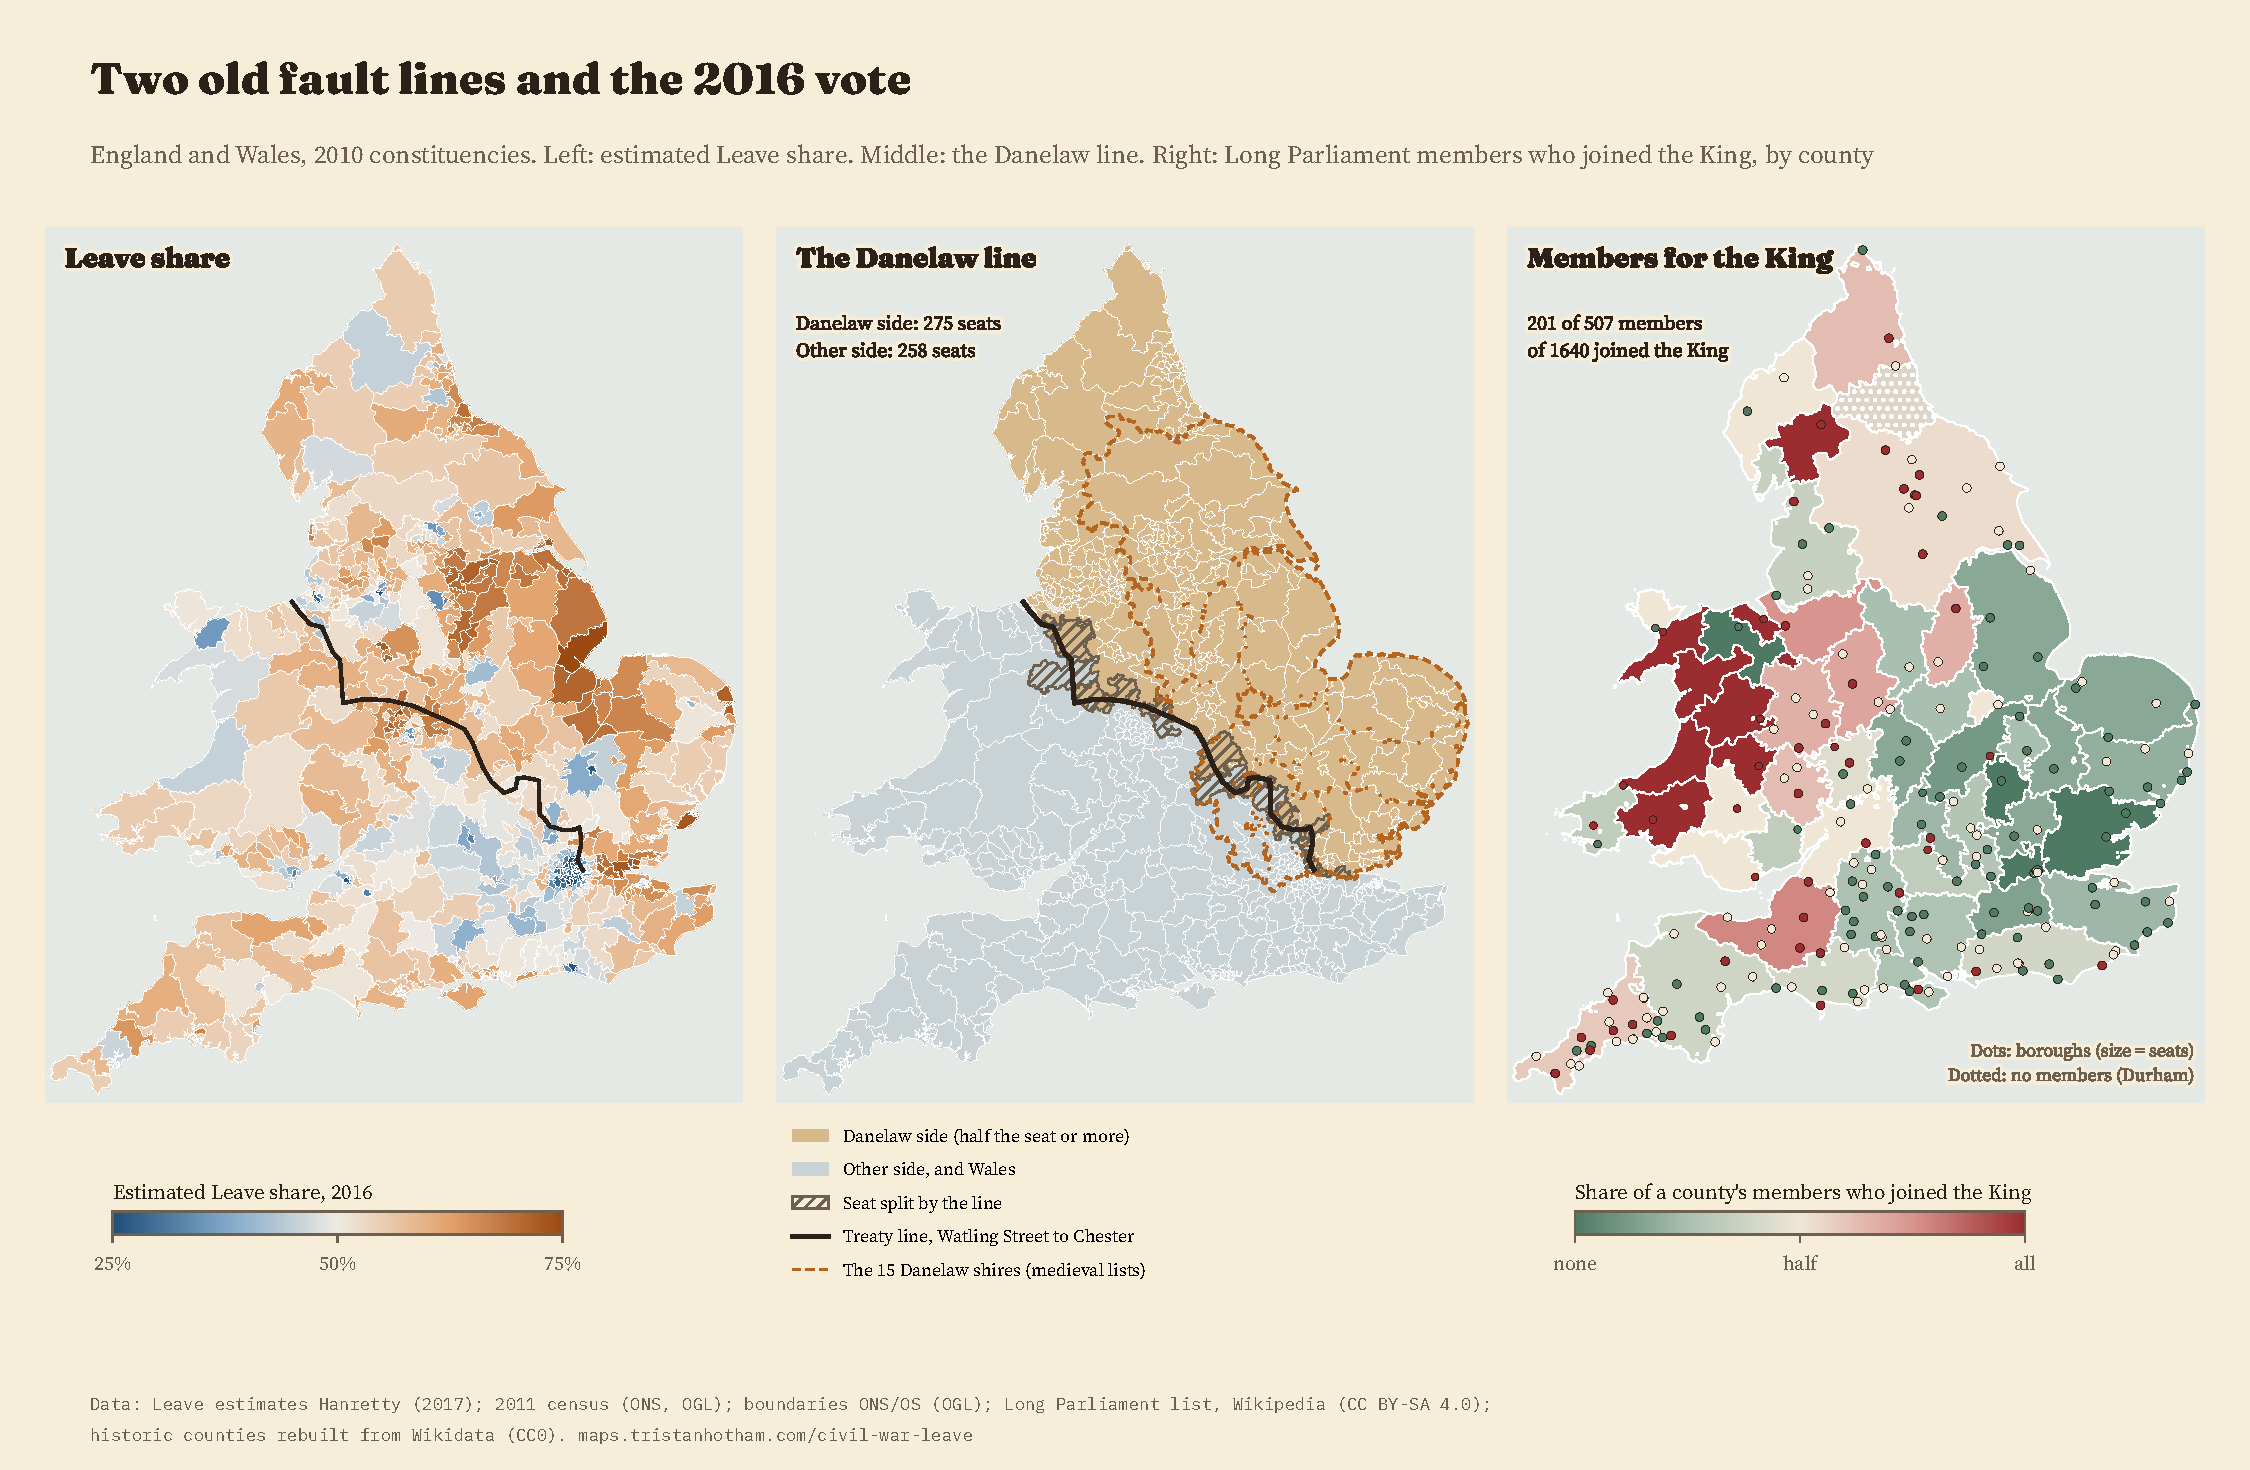
\includegraphics[width=\textwidth]{f_maps.pdf}
\caption{Left: estimated Leave share by 2010 constituency, England and Wales, with the Danelaw line. Middle: seats on each side of the line (hatched: split seats) and the fifteen Danelaw shires of the medieval lists (dashed). Right: share of each historic county's members of 1640 who later joined the King, with the 1640 boroughs as dots.}\label{fig:maps}\end{figure}

\subsection{Civil War allegiance}
The list of members elected to the Long Parliament in 1640 \citep{wiki1640} gives, for each of 267 constituencies grouped by county, the members returned and a notes column recording what happened to them: deaths, elevations to the peerage, void elections, expulsions and disablements. I parse every row. A member is coded as having joined the King when the notes say he was disabled, counting members elected at by-elections before the war and rows where both members were disabled. Ten hand decisions are recorded in the code: five disablements that did not reflect royalism are removed (Henry Marten, disabled for words against the King and later readmitted; the two Hothams, parliamentarians disabled for plotting to surrender Hull; a disablement of 1648; and Sir Ralph Verney, disabled in 1645 for refusing the Covenant), and five members who were killed fighting for the King before they could be disabled are added. Pre-war expulsions, such as those of monopolists in 1641, are not counted. The result is 201 of 507 seats (39.6\%) held by members who joined the King. For Wales without Monmouthshire the coding gives 17 of 24, the same as the count reported by \citet{dodd1952}. A national total from \citet{brunton1954} could not be consulted for this study, which is a limitation of the check.

Each historic county receives the share of its members (county and borough seats together) who joined the King. Shares range from none in 4 counties (Bedfordshire, Denbighshire, Essex and Middlesex) to all members in 8 (seven Welsh counties and Westmorland); 17 of 51 counties had a royalist majority among their members. Each 2010 seat takes the value of the historic county containing its reference point. As an exploratory measure, the 216 borough and university constituencies were placed at their towns and seats containing one were given the royalist share of its members.

\section{Research design}\label{sec:design}
\subsection{Analysis plan}
The plan was written in the study notes, with a timestamp, before any association between an exposure and an outcome was computed. At that point I had looked at the column names of the data, a single example row and the layout of the member lists. The plan fixed the hypotheses, the unit, the outcome, the exposures, the controls, the main specifications, the robustness checks, the inference and the smallest effect of interest, and a decision rule for the allegiance coding: it would count as usable for a planned test if at least 90\% of rows parsed and the total of royalists was within 25\% of a published count. All rows parsed; the published national count could not be consulted, so the check was replaced by the Welsh count, which the coding matches. This deviation is recorded in the notes. Everything reported as exploratory below was added after the planned analyses were run.

\subsection{Main specifications}
For Test 1 the main specification (M4) is
\begin{equation}
\text{Leave}_i = \beta\,\text{Danelaw}_i + \alpha_{r(i)} + f(\log \text{density}_i) + \gamma \log(1+\text{km to city}_i) + \mathbf{x}_i'\boldsymbol\delta + \varepsilon_i,
\end{equation}
estimated by OLS on the 533 English seats, where $\alpha_r$ are region fixed effects, $f$ is a natural cubic spline with four degrees of freedom and $\mathbf{x}_i$ are the eleven census shares. Standard errors are clustered by local authority district (the district containing most of the seat), because the Leave estimates distribute counted district results to seats \citep{hanretty2017,cameron2015}. The model ladder reports M1 (no controls), M2 (region), M3 (region and rurality) and M4; the full coefficients of M4 for both tests are in Table~\ref{tab:full}. Test 2 uses the same specification with the royalist share (per 10 points) in place of the Danelaw indicator, on England and Wales with Wales as a region, and with standard errors clustered by historic county, the level at which the exposure varies. With 49 clusters I also report wild cluster bootstrap p-values with Webb weights and the null imposed \citep{cameron2008,webb2023}, and a permutation test that shuffles the county values across counties. Holm-adjusted p-values are given for the two planned main coefficients \citep{holm1979}, and equivalence is assessed with two one-sided tests against the smallest effect of interest \citep{lakens2017}.

\subsection{Boundary design}
The second estimate for Test 1 compares seats either side of the line. On seats within 50 km of the land line, I estimate
\begin{equation}
\text{Leave}_i = \tau\,\text{Side}_i + \lambda_1 d_i + \lambda_2 \text{Side}_i\, d_i + \mu_{s(i)} + \mathbf{z}_i'\boldsymbol\theta + \varepsilon_i,
\end{equation}
where $d_i$ is the signed distance, $\mu_s$ are line-segment fixed effects and $\mathbf{z}_i$ are the rurality and census controls. The planned variants are bandwidths of 25 and 75 km, triangular kernel weights, no controls, region fixed effects instead of segment effects, and seats south of 52.75\textdegree{}N only, where the line follows the treaty text and the best attested part of Watling Street. Covariate balance at the line is checked by using each control in turn as the outcome, and placebo lines translated 50 km to either side test for jumps where there is no line. The same model with the Scandinavian name share as the outcome checks that the line marks a real historical difference. Boundary designs require that nothing else changes at the line \citep{eggers2015}; the balance checks speak to that directly.

\subsection{What the design can and cannot identify}
This is an observational, cross-sectional design. Neither exposure was assigned at random, and both are correlated with the geography of England: the Danelaw side is the north and east, and the royalist counties are concentrated in Wales, the west and the north. Region fixed effects absorb broad differences, but they also absorb much of the variation in the exposures. For the Danelaw, only 5 of the nine English regions contain seats on both sides of the line (the East Midlands, East of England, London, South East and West Midlands); the North East, North West and Yorkshire and the Humber lie wholly on the Danelaw side, and the South West wholly on the other. The main estimate is therefore identified from comparisons within those five regions, and in London from the eleven seats east of the Lea. The census controls are measured long after the exposures, so M4 asks whether the old line adds anything beyond the present composition of places, not whether it had a total effect; M2 is reported as the closest available estimate of the total association within regions.

\section{Results}\label{sec:results}
\subsection{Test 1: the Danelaw}
Seats on the Danelaw side had a mean estimated Leave share of 56.9\%, against 50.0\% on the other side, a raw gap of 6.9 points. Table~\ref{tab:t1} and Figure~\ref{fig:ladder} show how the gap changes as controls are added. With region fixed effects it is 8.01 points (95\% CI 2.82 to 13.19), driven largely by London, where the eleven Danelaw seats east of the Lea had a mean Leave share of 52.6\% against 38.0\% in the rest of the capital. Adding density and distance to a city leaves 6.70 points. Adding the census composition removes the gap entirely: the main estimate is -0.16 points (95\% CI -1.81 to 1.49; $p$ = 0.85; N = 533; 305 clusters). The 90\% interval (-1.54 to 1.22) is not entirely inside $\pm1$ point, so the result is not formally equivalent to zero at the planned threshold ($p$ = 0.16), but the point estimate is close to zero and the interval excludes the raw gap by a wide margin. Spatial standard errors give narrower intervals (Conley, 100 km: -1.03 to 0.71).

\begin{table}[tbp]\centering\footnotesize\caption{Test 1. Leave share and the Danelaw side of the line (England): model ladder.}\label{tab:t1}\begin{tabular}{llrrrrrr}\toprule Model & Controls & $\beta$ (points) & SE & 95\% CI & N & Clusters & $R^2$\\\midrule
M1 & No controls & $6.88^{***}$ & (1.30) & (4.32, 9.44) & 533 & 305 & 0.10\\
M2 & Region FE & $8.01^{**}$ & (2.64) & (2.82, 13.19) & 533 & 305 & 0.32\\
M3 & Region FE + rurality & $6.70^{***}$ & (1.86) & (3.03, 10.36) & 533 & 305 & 0.49\\
M4 & + composition (main) & $-0.16$ & (0.84) & (-1.81, 1.49) & 533 & 305 & 0.91\\
\bottomrule\end{tabular}\par\vspace{0.3em}\parbox{0.92\textwidth}{\scriptsize OLS. Outcome: estimated Leave share (\%). Exposure: at least half the seat's area on the Danelaw side. Rurality: natural cubic spline (4 df) of log density and log(1 + km to a city of 100,000+). Composition: the eleven census shares in Table~\ref{tab:desc}. Standard errors clustered by local authority. $^{*}p<0.05$, $^{**}p<0.01$, $^{***}p<0.001$.}\end{table}

\begin{figure}[tbp]\centering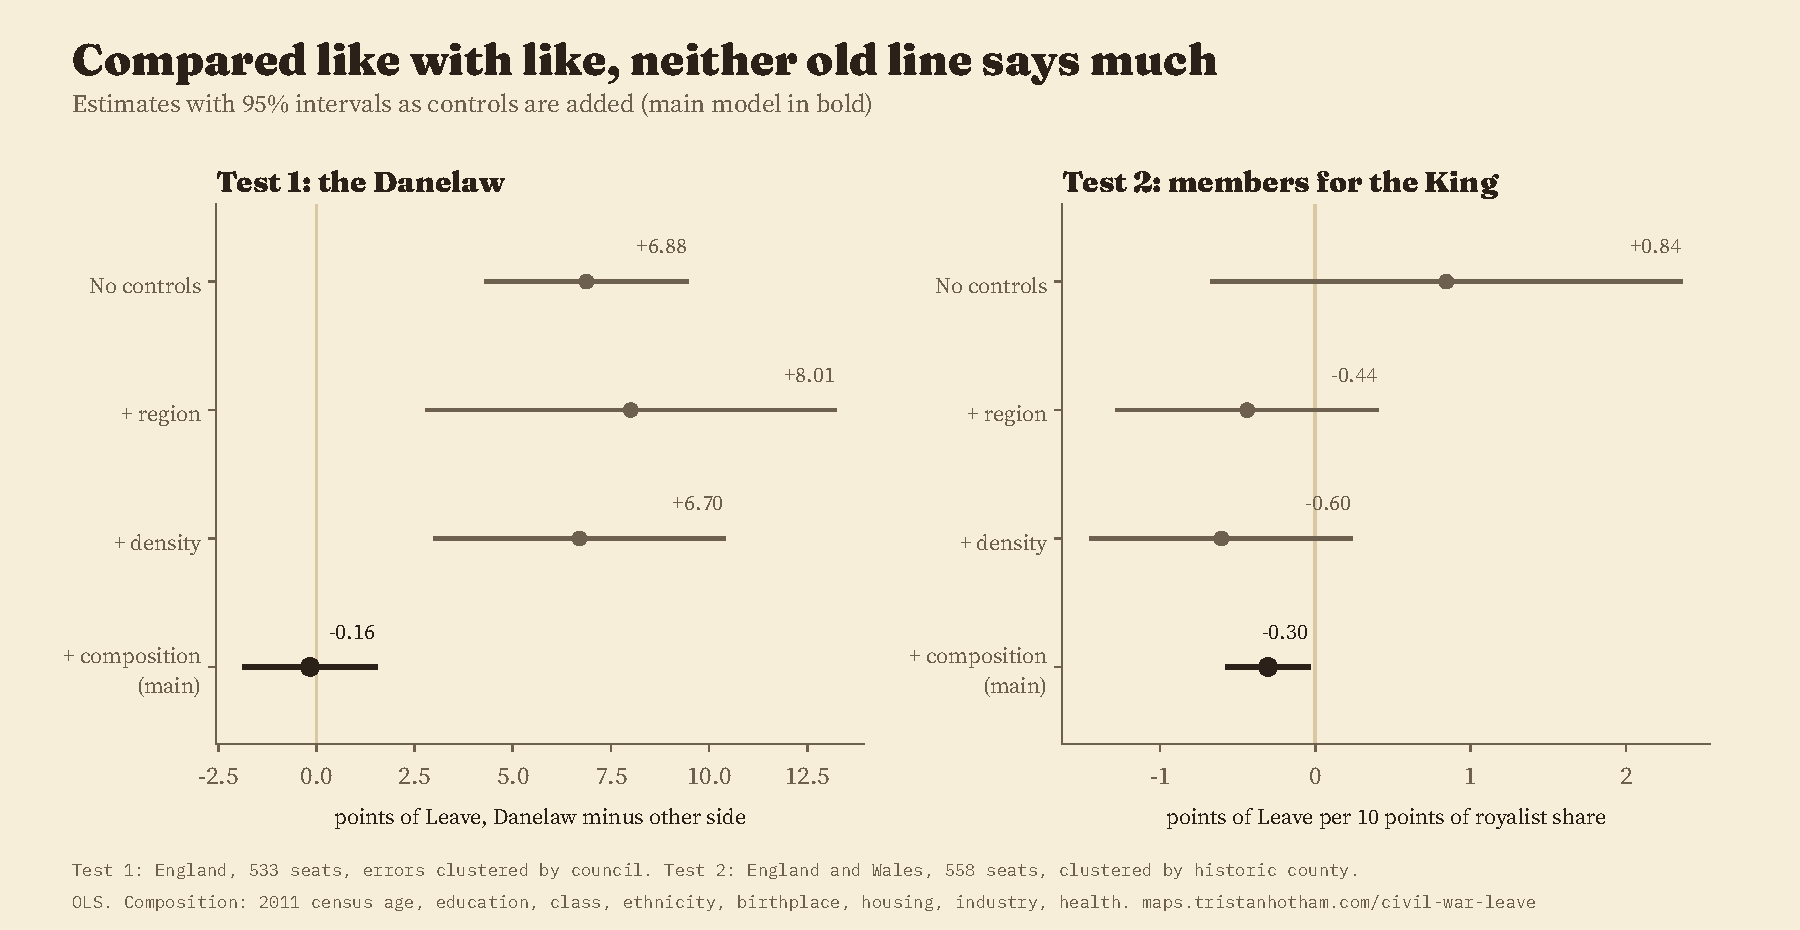
\includegraphics[width=\textwidth]{f_ladder.pdf}
\caption{Model ladders for the two tests: estimates with 95\% confidence intervals as controls are added. Test 1: Leave share, Danelaw side minus other side (points). Test 2: Leave share per 10 points of the county's royalist share.}\label{fig:ladder}\end{figure}

The raw gap is accounted for by differences in composition that are large and familiar from the Leave literature. Danelaw seats in England had on average 10.3 points more White British residents, 6.5 points fewer residents with a degree-level qualification and 7.6 points fewer born abroad than seats on the other side. These are among the strongest predictors of the Leave vote \citep{becker2017,goodwin2016}.

\subsection{The boundary design}
Figure~\ref{fig:line} shows the Leave share and the Scandinavian name share of seats within 50 km of the line. The raw Leave share rises across the line, but it is also falling towards the line on the English side, because the seats closest to it on that side include the London boroughs west of the Lea and the cities of the Ouse and Watling Street corridor. With controls, the jump at the line is -0.42 points (95\% CI -3.34 to 2.50; N = 251). Table~\ref{tab:rd} shows that the estimate is unstable: 3.65 points at 25 km ($p$ = 0.04), -2.13 at 75 km, 1.24 with triangular weights and 9.60 without controls. The placebo line 50 km to the north-east shows no jump (-0.12), but the placebo line 50 km to the south-west shows one of 2.59 points (95\% CI 0.14 to 5.05), where there is no historical boundary at all.

\begin{figure}[tbp]\centering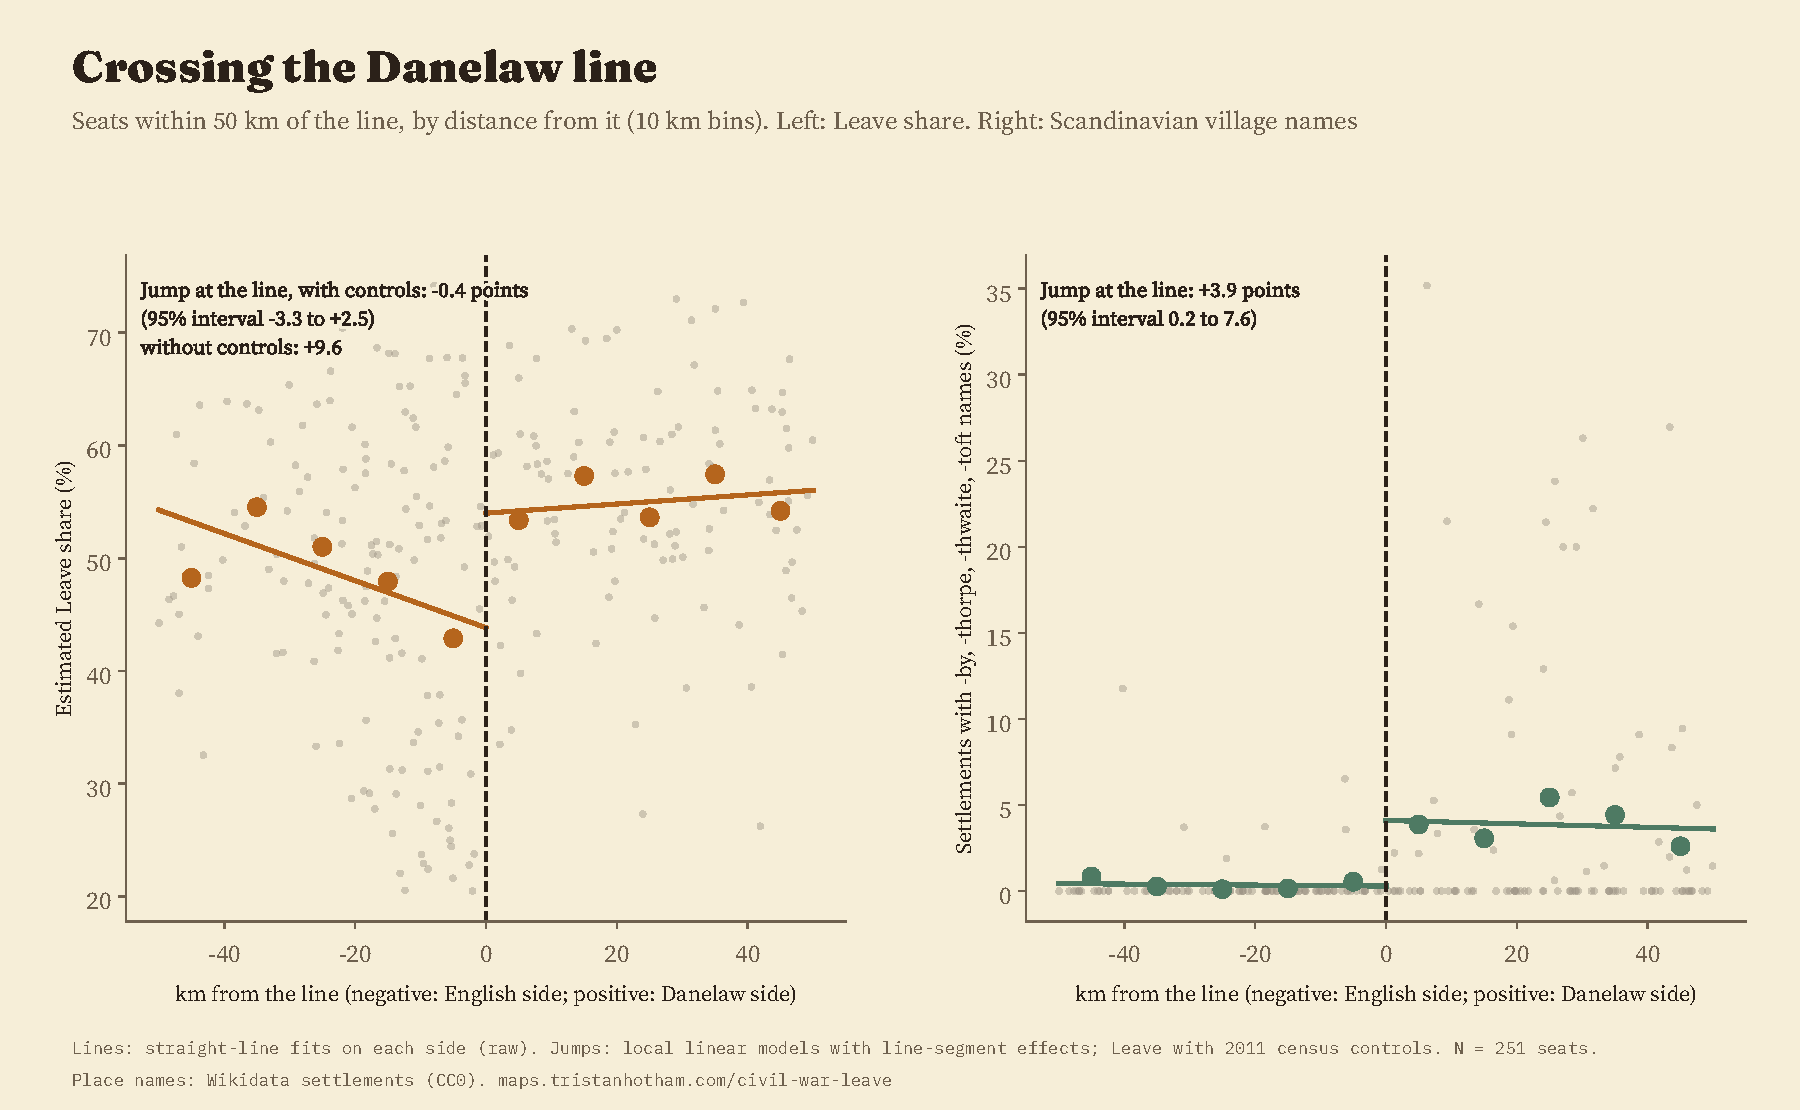
\includegraphics[width=\textwidth]{f_line.pdf}
\caption{Seats within 50 km of the Danelaw line by signed distance from it (negative: English side). Grey: seats; coloured: 10 km bin means; lines: straight-line fits on each side. Left: estimated Leave share. Right: share of settlements with Scandinavian name endings.}\label{fig:line}\end{figure}

\begin{table}[tbp]\centering\scriptsize\caption{Boundary design: the jump in Leave share at the Danelaw line.}\label{tab:rd}\begin{tabular}{lrrrrrr}\toprule Specification & Jump & 95\% CI & $p$ & Danelaw side & Other & Clusters\\\midrule
Main: 50 km, segment FE, controls & $-0.42$ & (-3.34, 2.50) & 0.778 & 106 & 145 & 141\\
25 km & $3.65^{*}$ & (0.23, 7.07) & 0.037 & 53 & 107 & 81\\
75 km & $-2.13$ & (-4.74, 0.48) & 0.109 & 158 & 173 & 194\\
Triangular kernel, 50 km & $1.24$ & (-1.71, 4.18) & 0.407 & 106 & 145 & 141\\
No controls & $9.60^{*}$ & (2.02, 17.19) & 0.013 & 106 & 145 & 141\\
Region FE in place of segment FE & $0.84$ & (-1.82, 3.51) & 0.533 & 106 & 145 & 141\\
South of 52.75 N only & $1.68$ & (-1.22, 4.58) & 0.254 & 54 & 144 & 114\\
Placebo line 50 km north-east & $-0.12$ & (-2.64, 2.41) & 0.927 & 82 & 101 & 110\\
Placebo line 50 km south-west & $2.59^{*}$ & (0.14, 5.05) & 0.039 & 132 & 47 & 106\\
Outcome: Scandinavian name share (no controls) & $3.90^{*}$ & (0.15, 7.64) & 0.042 & 96 & 92 & 118\\
\bottomrule\end{tabular}\par\vspace{0.3em}\parbox{0.92\textwidth}{\scriptsize Local linear in signed distance with separate slopes each side, seats within the bandwidth of the land line (Lea to Chester), England. Line-segment fixed effects and the rurality and composition controls unless stated. Placebo lines: whole line translated 50 km perpendicular to its direction; only seats on the same side of the real line. Standard errors clustered by local authority.}\end{table}

The reason is visible in the balance checks (Figure~\ref{fig:balance}). At the line, 7 of the 13 control variables jump significantly when used as outcomes: the Danelaw side of the line is less dense (-0.78 standard deviations in log density), further from a city (0.86), less likely to hold a degree (-0.64) and less likely to rent socially (-0.78). The line runs along the edge of London and the cities of the Midlands, so it separates urban from less urban places. A boundary design cannot separate a historical effect from that contrast. By contrast, the share of Scandinavian place-names jumps at the line by 3.9 points (95\% CI 0.2 to 7.6) from almost none on the English side. The line marks a real historical difference in settlement; it does not mark a difference in the Leave vote that survives comparison of like with like.

\begin{figure}[tbp]\centering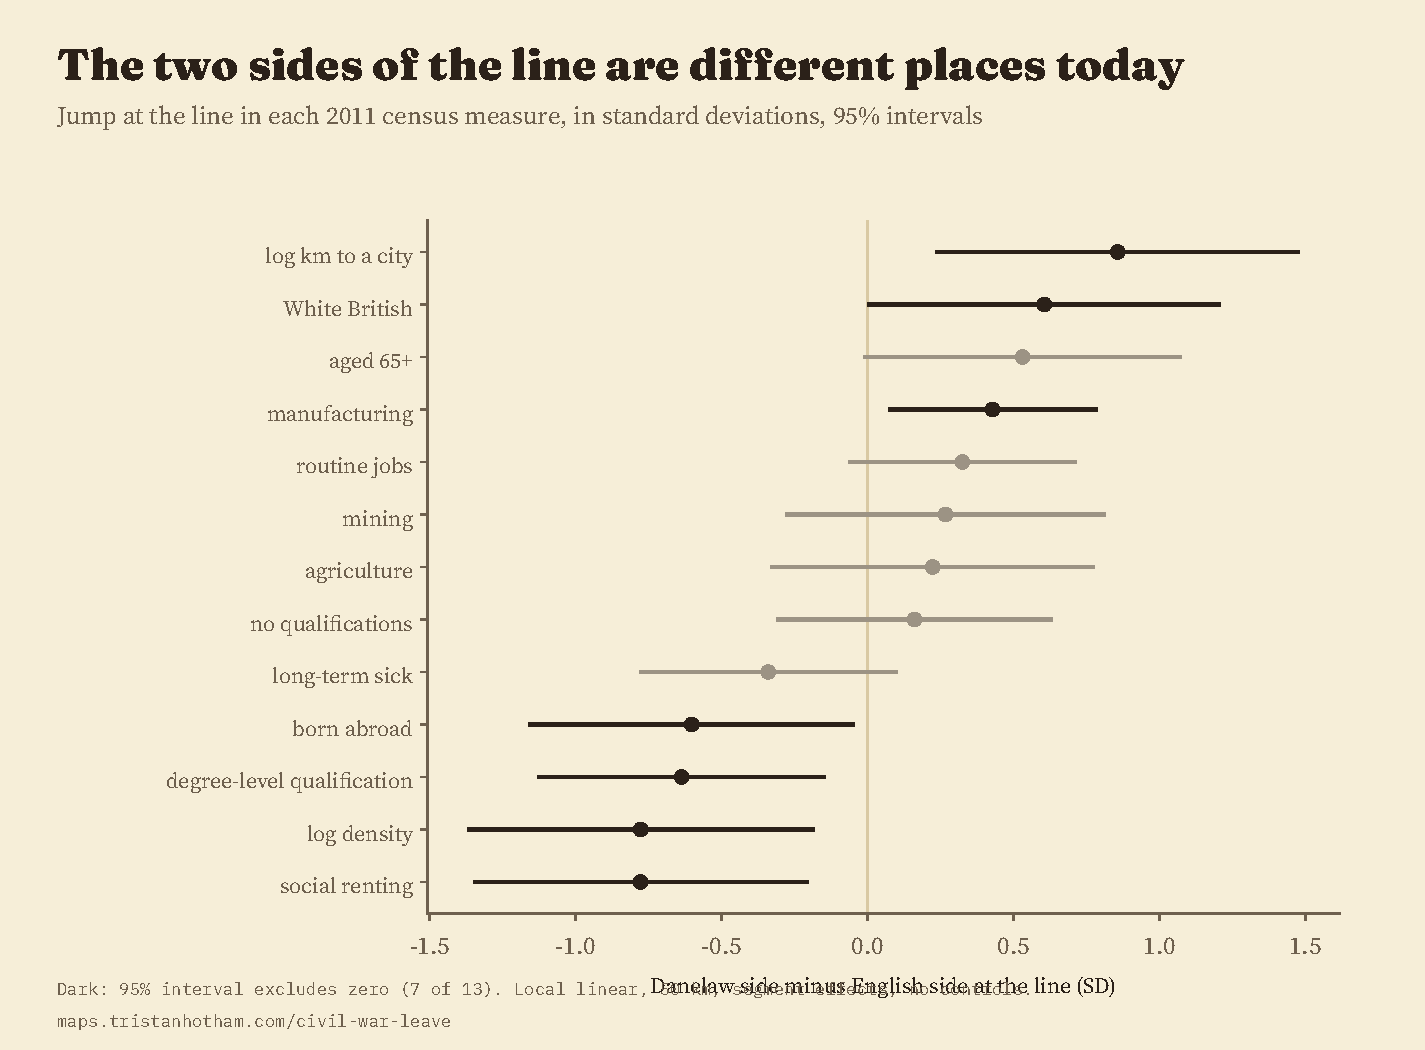
\includegraphics[width=0.78\textwidth]{f_balance.pdf}
\caption{Covariate balance at the Danelaw line: the jump in each control at the line, in standard deviations, from the boundary model without controls (50 km, segment effects). Dark: 95\% interval excludes zero.}\label{fig:balance}\end{figure}

\subsection{Other measures of the Danelaw}
The area share version of D1 gives -0.05 points per 10 points of area (95\% CI -0.23 to 0.14), and the Scandinavian name share gives -0.34 points per 10 points (95\% CI -0.92 to 0.24). The one measure that differs is D2, the fifteen shires of the medieval lists: seats in those shires had a Leave share 2.07 points higher than other seats with the same controls (95\% CI 0.64 to 3.50). This coding differs from the line mainly in the north, where the shire lists leave out Lancashire, Cumberland, Westmorland, Northumberland and Durham, and around London, where they include Middlesex and Buckinghamshire. I do not read it as support for H1. It is one of ten planned checks, the measure that corresponds to the treaty shows nothing, and the shire coding contrasts the north-west and north-east with Yorkshire and the East Midlands within regions where those areas are known to differ in many ways. What it does show is that the answer depends on which Danelaw one draws, a reason to treat any single map comparison with caution.

\subsection{Test 2: Civil War allegiance}
Table~\ref{tab:t2} reports the ladder for the royalist share. Without controls, seats in counties with more royalist members had a slightly higher Leave share, 0.84 points per 10 points of royalist share (95\% CI -0.66 to 2.35), not distinguishable from zero. With region fixed effects the sign turns negative (-0.44), and in the main specification the estimate is -0.30 points per 10 points (95\% CI -0.56 to -0.05; $p$ = 0.021; N = 558; 49 counties), or -0.72 points per standard deviation of royalist share. The wild cluster bootstrap p-value is 0.069 (9,999 draws), above the conventional threshold; the permutation test, which shuffles county values across counties, gives 0.005. The Holm-adjusted p-value across the two planned main coefficients is 0.042. The 90\% interval per standard deviation (-1.23 to -0.21) is not inside $\pm1$ point, so equivalence to zero is not established either.

\begin{table}[tbp]\centering\scriptsize\caption{Test 2. Leave share and the share of the county's members of 1640 who joined the King (England and Wales): model ladder.}\label{tab:t2}\begin{tabular}{llrrrrrrr}\toprule Model & Controls & $\beta$ (per 10 pts) & SE & 95\% CI & per SD & N & Clusters & $R^2$\\\midrule
M1 & No controls & $0.844$ & (0.750) & (-0.66, 2.35) & 2.01 & 558 & 49 & 0.03\\
M2 & Region FE & $-0.438$ & (0.416) & (-1.27, 0.40) & -1.04 & 558 & 49 & 0.28\\
M3 & Region FE + rurality & $-0.604$ & (0.416) & (-1.44, 0.23) & -1.44 & 558 & 49 & 0.47\\
M4 & + composition (main) & $-0.303^{*}$ & (0.127) & (-0.56, -0.05) & -0.72 & 558 & 49 & 0.91\\
\midrule\multicolumn{9}{l}{Inference for the main model: wild cluster bootstrap $p$ = 0.069 (M2: 0.418); permutation $p$ = 0.005; Holm-adjusted $p$ = 0.042}\\
\bottomrule\end{tabular}\par\vspace{0.3em}\parbox{0.92\textwidth}{\scriptsize OLS, controls as in Table~\ref{tab:t1} with Wales as a region. Standard errors clustered by historic county (49 counties). Wild cluster bootstrap: Webb six-point weights, null imposed, 9,999 draws. Permutation: county values shuffled across counties, 5,000 draws.}\end{table}

Figure~\ref{fig:county} shows the county-level picture. In the raw data, Middlesex, which had no royalist members, had the lowest mean Leave share of any county (37.0\%). After adjustment, Middlesex sits close to zero (-0.12 points), and the slope through the adjusted county means is gently negative. The correlation between county mean Leave and royalist share is -0.07 in the raw data.

\begin{figure}[tbp]\centering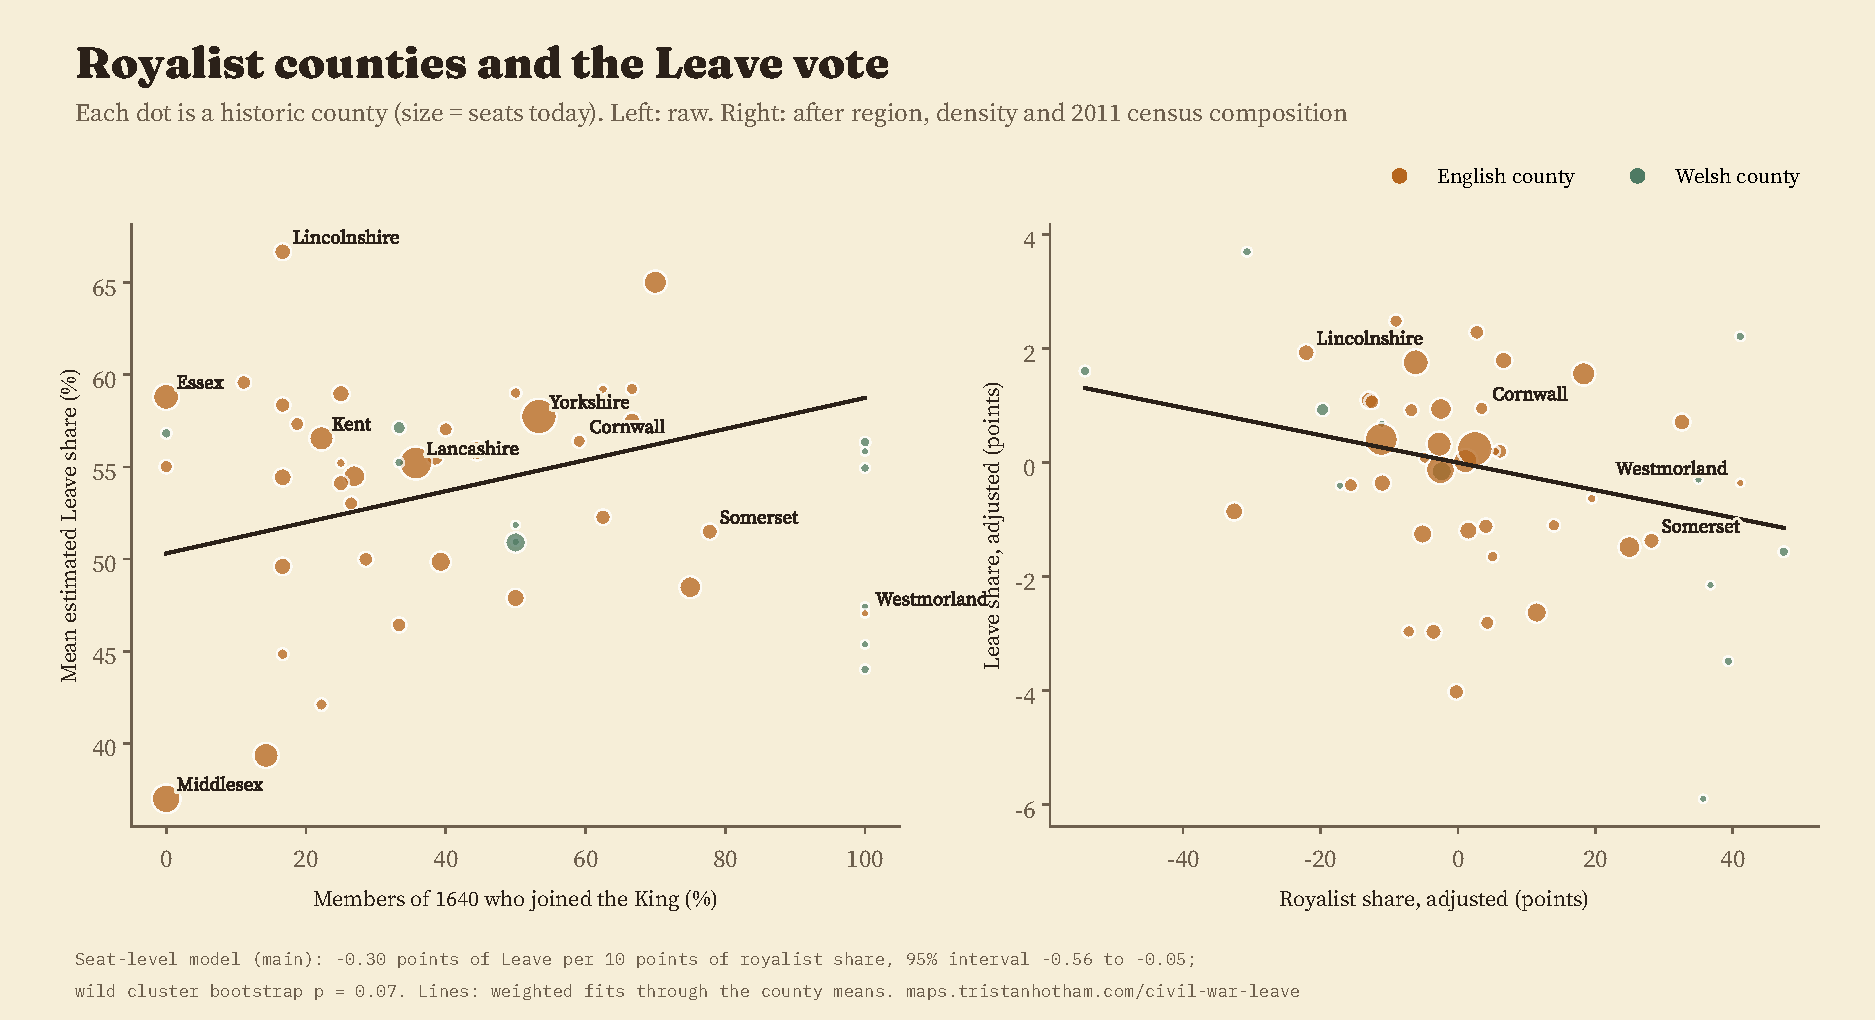
\includegraphics[width=\textwidth]{f_county.pdf}
\caption{Historic counties of England and Wales: share of members of 1640 who joined the King against the mean Leave share of their 2010 seats. Left: raw. Right: both adjusted for region, density and 2011 census composition (seat-level residuals averaged by county). Dot size: number of seats.}\label{fig:county}\end{figure}

\section{Robustness}\label{sec:robust}
\subsection{Test 1}
Figure~\ref{fig:forest} and Table~\ref{tab:rob1} report every planned check. Apart from the shire coding, none of the 10 checks finds a significant gap: not the seats south of 52.75\textdegree{}N (-0.14), not the seats with counted ward results (-0.63, N = 112), not dropping London (-0.99), not density decile fixed effects, not adding Wales as a non-Danelaw nation, not dropping influential seats and not clustering by historic county. Leaving out each region in turn gives estimates from -0.99 to 0.90, none significant. For the other outcomes, the Danelaw indicator has no significant association with UKIP's 2015 vote share (0.50), the Brexit Party's 2019 share in the seats it contested (-0.35) or Reform UK's 2024 share mapped onto 2010 seats (-0.85).

\begin{figure}[tbp]\centering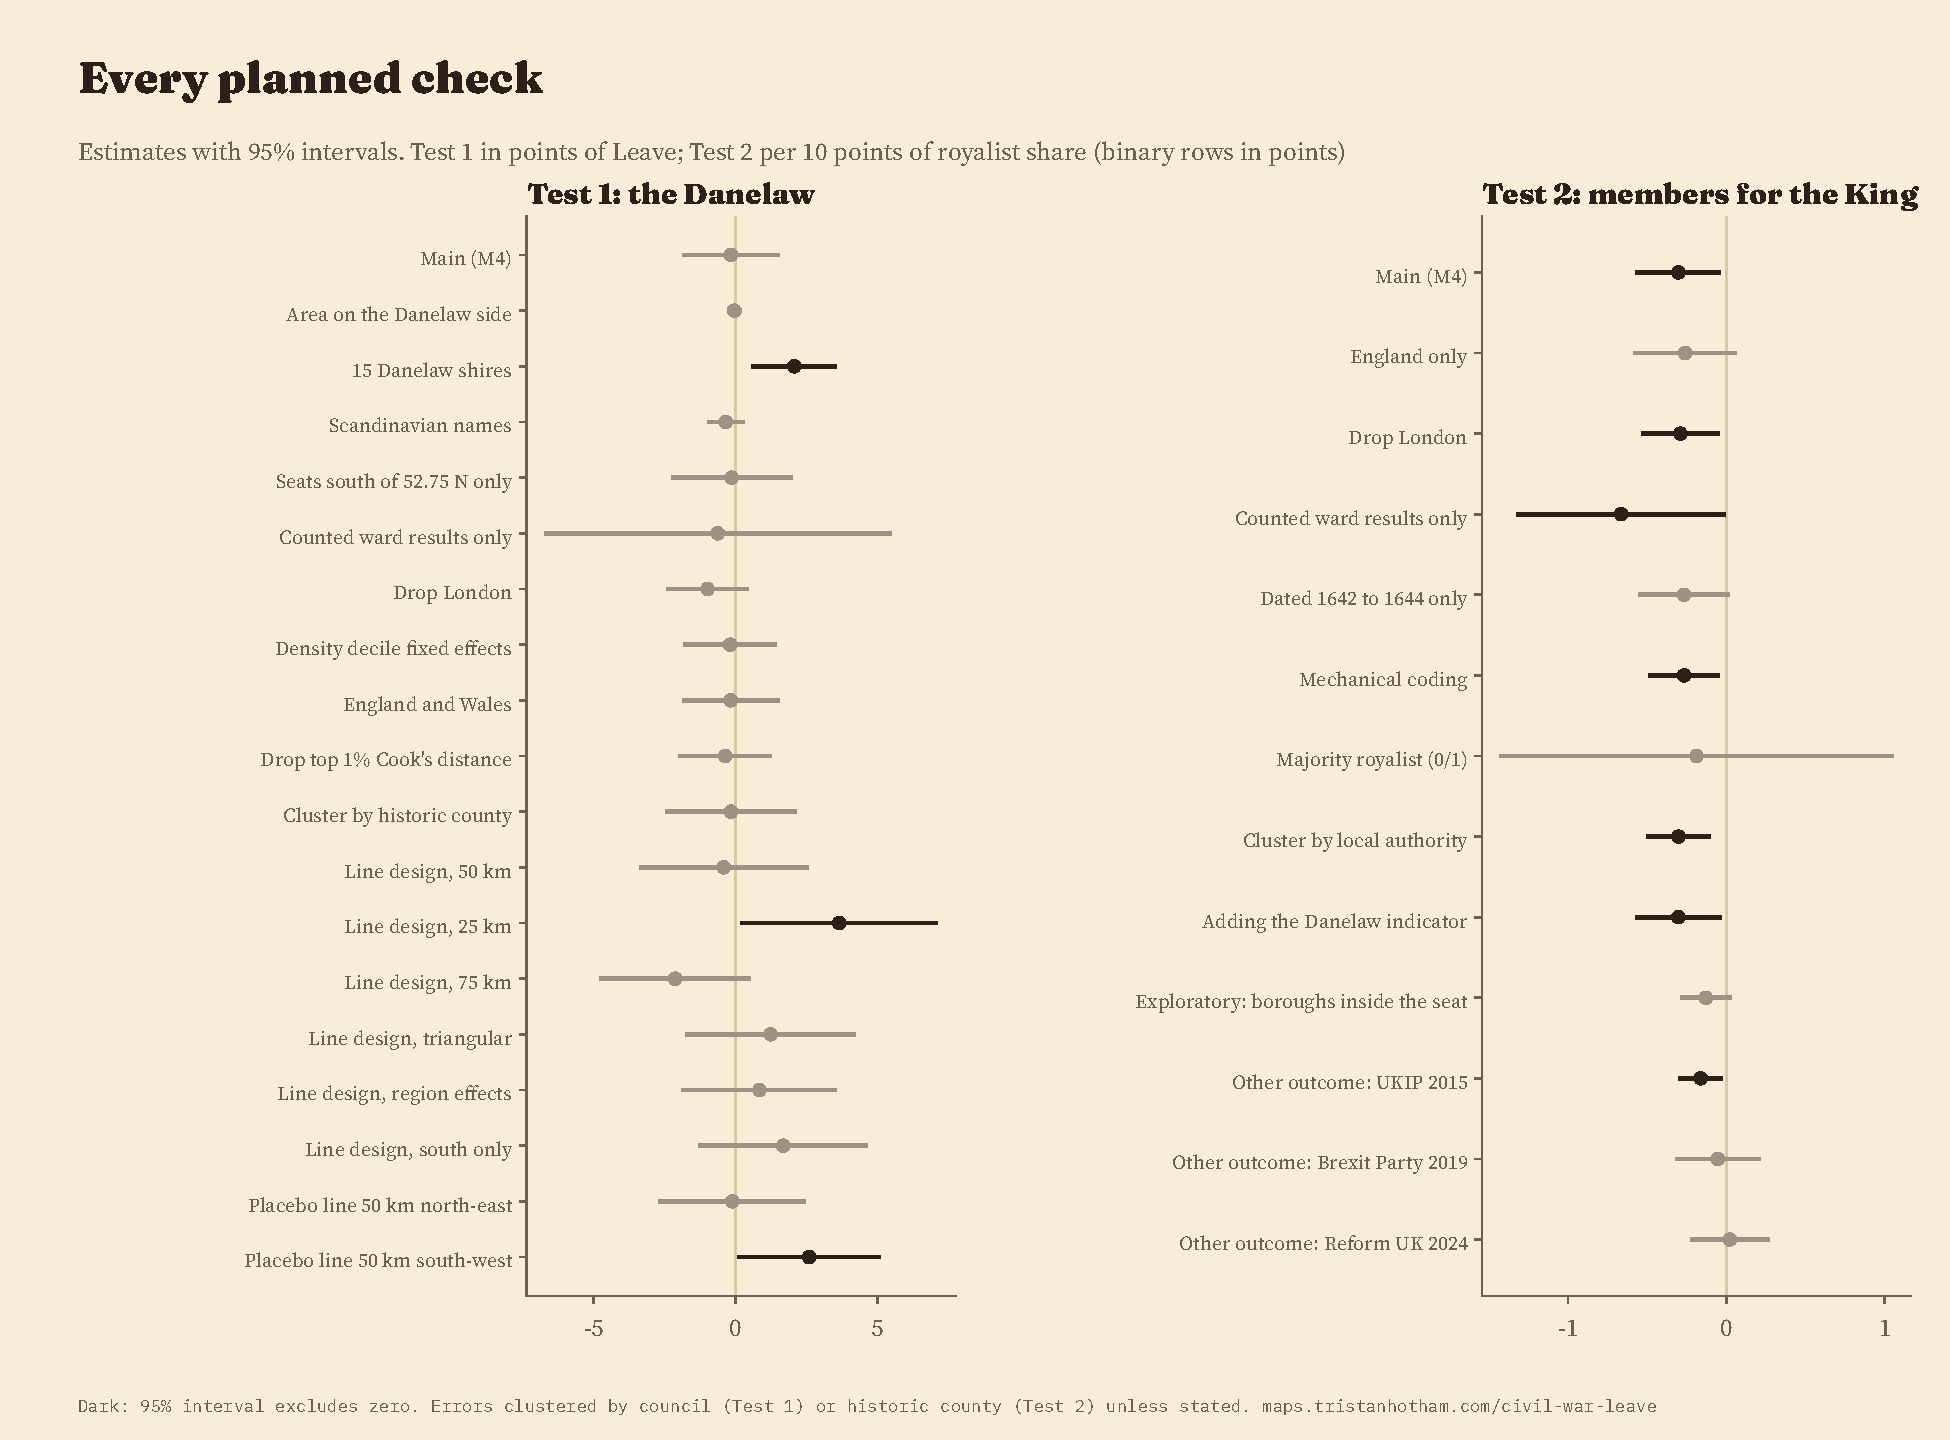
\includegraphics[width=\textwidth]{f_forest.pdf}
\caption{Every planned check for both tests, with 95\% confidence intervals. Dark: interval excludes zero. Test 1 in points of Leave (area share and Scandinavian names per 10 points); Test 2 per 10 points of royalist share (the majority indicator in points).}\label{fig:forest}\end{figure}

\begin{table}[tbp]\centering\scriptsize\caption{Test 1 robustness and measurement checks (all planned).}\label{tab:rob1}\begin{tabular}{p{7.4cm}rrrrr}\toprule Specification & $\beta$ & 95\% CI & $p$ & N & Clusters\\\midrule
Main specification (M4) & $-0.161$ & (-1.81, 1.49) & 0.847 & 533 & 305\\
Exposure: share of seat area on the Danelaw side (per 10 points) & $-0.047$ & (-0.23, 0.14) & 0.619 & 533 & 305\\
Exposure: the 15 Danelaw shires of the medieval shire lists & $2.070^{**}$ & (0.64, 3.50) & 0.005 & 533 & 305\\
Exposure: Scandinavian place-name share (per 10 points) & $-0.340$ & (-0.92, 0.24) & 0.250 & 469 & 282\\
Seats south of 52.75 N only & $-0.138$ & (-2.20, 1.93) & 0.896 & 332 & 204\\
Counted ward results only & $-0.627$ & (-6.68, 5.43) & 0.836 & 112 & 51\\
Drop London & $-0.986$ & (-2.37, 0.40) & 0.162 & 460 & 273\\
Density decile fixed effects & $-0.190$ & (-1.77, 1.39) & 0.814 & 533 & 305\\
England and Wales (Wales outside the Danelaw) & $-0.170$ & (-1.81, 1.47) & 0.839 & 573 & 327\\
Drop top 1\% Cook's distance & $-0.370$ & (-1.95, 1.21) & 0.646 & 527 & 304\\
Cluster by historic county & $-0.161$ & (-2.40, 2.07) & 0.885 & 533 & 38\\
Outcome: UKIP 2015 & $0.500$ & (-0.57, 1.57) & 0.357 & 533 & 305\\
Outcome: Brexit Party 2019 (seats contested) & $-0.355$ & (-1.91, 1.20) & 0.652 & 228 & 123\\
Outcome: Reform UK 2024 (approximate) & $-0.855$ & (-1.98, 0.27) & 0.137 & 533 & 305\\
\bottomrule\end{tabular}\par\vspace{0.3em}\parbox{0.92\textwidth}{\scriptsize Points of Leave for indicators; per 10 points for the area share and the Scandinavian name share. Standard errors clustered by local authority unless stated.}\end{table}

\subsection{Test 2}
The negative estimate for the royalist share is consistent in sign but not in significance (Table~\ref{tab:rob2}). It is significant when London is dropped (-0.29), when errors are clustered by local authority instead of county (-0.30, which understates the dependence), with the purely mechanical coding without hand decisions (-0.27) and with counted ward results (-0.66, N = 108). It is not significant for England alone (-0.26, $p$ = 0.10), when only disablements dated 1642 to 1644 are counted (-0.27, $p$ = 0.06), or with a simple indicator of a royalist majority among a county's members (-0.19 points, 95\% CI -1.42 to 1.04). Leaving out each region (Table~\ref{tab:loro}) gives -0.47 to -0.26 (8 of 10 significant), and leaving out each county gives -0.44 to -0.25. UKIP's 2015 share shows a similar small negative association (-0.16, 95\% CI -0.29 to -0.03); the Brexit Party in 2019 (-0.05) and Reform UK in 2024 (0.02) show none. The exploratory seat-level measure, the royalist share of the members of a 1640 borough inside the seat, gives -0.13 (95\% CI -0.28 to 0.02; N = 149). Adding the Danelaw indicator does not change the estimate (-0.30).

\begin{table}[tbp]\centering\scriptsize\caption{Test 2 robustness checks (planned unless marked exploratory).}\label{tab:rob2}\begin{tabular}{p{7.4cm}rrrrr}\toprule Specification & $\beta$ & 95\% CI & $p$ & N & Clusters\\\midrule
Main specification (M4) & $-0.303^{*}$ & (-0.56, -0.05) & 0.021 & 558 & 49\\
England only & $-0.261$ & (-0.57, 0.05) & 0.097 & 518 & 37\\
Drop London (Middlesex and Surrey seats in London) & $-0.291^{*}$ & (-0.52, -0.06) & 0.016 & 485 & 49\\
Counted ward results only & $-0.664^{*}$ & (-1.31, -0.02) & 0.045 & 108 & 20\\
Exposure: disablements dated 1642 to 1644 only & $-0.268$ & (-0.55, 0.01) & 0.058 & 558 & 49\\
Exposure: every disablement, no hand decisions & $-0.267^{*}$ & (-0.48, -0.06) & 0.014 & 558 & 49\\
Exposure: majority of the county's members royalist (0/1) & $-0.189$ & (-1.42, 1.04) & 0.759 & 558 & 49\\
Cluster by local authority & $-0.303^{**}$ & (-0.49, -0.11) & 0.002 & 558 & 322\\
Adding the Danelaw indicator & $-0.303^{*}$ & (-0.56, -0.05) & 0.022 & 558 & 49\\
Exploratory: royalist share of a 1640 borough inside the seat (seats with one) & $-0.130$ & (-0.28, 0.02) & 0.083 & 149 & 128\\
Outcome: UKIP 2015 & $-0.162^{*}$ & (-0.29, -0.03) & 0.014 & 558 & 49\\
Outcome: Brexit Party 2019 (seats contested) & $-0.054$ & (-0.31, 0.20) & 0.670 & 246 & 40\\
Outcome: Reform UK 2024 (approximate) & $0.023$ & (-0.21, 0.26) & 0.847 & 558 & 49\\
\bottomrule\end{tabular}\par\vspace{0.3em}\parbox{0.92\textwidth}{\scriptsize Per 10 points of royalist share, except the majority indicator (points). Standard errors clustered by historic county unless stated; the exploratory borough measure by local authority.}\end{table}

\section{Discussion}\label{sec:disc}
\subsection{What the results show}
Neither old division of England adds much to what the present-day composition of places explains about the Leave vote. For the Danelaw the planned specification finds no association, although the equivalence test at one point does not pass: the raw gap of 6.9 points is entirely accounted for by region, density and composition, the estimate is close to zero, and the main planned checks agree. The boundary design does not rescue the claim; it shows that the line separates places that differ today in density and education, and that comparable jumps can be found where there is no line. The place-names show that the line is not imaginary. It marks a difference in the density of Scandinavian settlement names that is visible more than a thousand years later. That difference simply does not carry over into the Leave vote once like is compared with like.

For the Civil War the evidence is weaker in both directions. There is a small negative conditional association: seats in counties whose members were more royalist voted Leave slightly less, by about 0.7 points per standard deviation of royalist share, which is small relative to a standard deviation of the Leave share of about 11 points. It is the opposite of the reading that the Cavalier counties became the Leave heartlands, and it is fragile: the wild bootstrap does not reject zero at the 5\% level, and three planned checks lose significance. A reader who wants a single sentence should take away that the Civil War sides of the counties' members do not predict the Leave vote in any substantively important way.

\subsection{What the results do not show}
Several limits apply. First, controlling for 2011 composition asks whether the old divisions add anything beyond the places they helped to make. If the Danelaw or the Civil War shaped where people of different ages, education or origins live, that path is inside the controls, and the cross-section cannot separate it from confounding. The region-only estimates are the best available guide to the total association within regions: positive and sizeable for the Danelaw (8.01 points), driven largely by east London, and negative but not significant for the Civil War (-0.44).

Second, the measures are rough. The treaty line is attested only as far as Watling Street, and its continuation to Chester is a convention of modern maps; the boundary itself may have lasted no more than seven years \citep{rochester2023}. The legal Danelaw of the shire lists is a different area. Members of Parliament were drawn from the gentry, and a county's members are not a measure of the allegiance of its people or of the territory each side held. A territorial coding from a contemporary-style map of the districts held by each side in 1643 \citep{gardiner1914} would be a natural complement; I did not have such a map as data. The historic counties are rebuilt approximately from point data, and Yorkshire is treated as one county.

Third, the unit of analysis is large. Constituencies average about 100,000 people, and the boundary design has only 251 seats within 50 km of the line. Ward- or output-area-level Leave estimates and parish-level historical data would allow a finer test. The Leave estimates themselves are model-based for most seats \citep{hanretty2017}; restricting to seats with counted results leaves too few for precision.

Fourth, the absence of a conditional association does not mean that history is irrelevant to the referendum. It means that these two lines, as measured here, do not mark a difference in the vote that the usual demographic predictors miss. Other historical legacies, such as industrial history, which is more directly connected to the composition of places today, are more plausible candidates.

\subsection{Relation to other work}
The results fit the main finding of the aggregate literature on the referendum: a small set of present-day characteristics of places, above all education, age and ethnicity, explains most of the variation in the vote \citep{becker2017,goodwin2016,alabrese2019}. They also illustrate the general caution of the persistence literature: historical exposures correlated with present-day geography will appear to predict present-day outcomes unless that geography is held fixed, and spatially correlated data can make such associations look precise \citep{conley1999}. Studies that do find persistence, such as \citet{voigtlaender2012}, rest on a historical exposure that is specific to a group and an outcome that is closely related to it; a broad territorial line and a referendum on European Union membership have no such link. The comparison of maps that motivated this study is a vivid example. The two maps do resemble each other, and the resemblance is about where people of different kinds live today.

\section{Conclusion}
Two old fault lines of England, the Danelaw boundary agreed by Alfred and Guthrum and the division of the Long Parliament between King and Parliament, were tested against the 2016 Leave vote with a plan written in advance. Seats on the Danelaw side voted Leave by 6.9 points more, but compared with similar places in the same region the gap is -0.16 points; the line still marks a jump in Scandinavian place-names but not in the vote. Counties whose members sided with the King voted slightly less Leave once composition is held fixed, by an amount that is small and not robust. The resemblance between the referendum map and these old divisions is real, but it is a resemblance of places, not, on this evidence, a political memory.

\section*{Data availability statement}
Data and code: Zenodo DOI https://doi.org/10.5281/zenodo.24104516. The interactive map is at \url{https://maps.tristanhotham.com/civil-war-leave/} and the repository at \url{https://github.com/Tristan-Hotham/civil-war-leave}. \texttt{analysis.csv} holds every variable used in the models, \texttt{seat\_geo.csv} the Danelaw and county measures for each seat, \texttt{lp1640\_constituencies.csv} the parsed member list with every coding decision, \texttt{county\_allegiance.csv} the county shares, \texttt{danelaw\_line.geojson} the line, and \texttt{results.json} every number in this paper. Census and boundary data are Crown copyright (Open Government Licence v3.0); the member list derives from Wikipedia (CC BY-SA 4.0); Wikidata is CC0; text and figures CC BY 4.0; code MIT.

\section*{AI statement}
I wrote the text, with drafting and editing assistance from Claude (Anthropic), which also helped prepare the analysis code. I reviewed and checked all text and results.

\bibliographystyle{plainnat}
\bibliography{refs}

\appendix
\section{Full regression tables}\label{app:tables}
\begin{table}[tbp]\centering\tiny\caption{Full coefficient tables (outcome: estimated Leave share, \%).}\label{tab:full}\begin{tabular}{lrrrrrr}\toprule Term & T1 M1 & T1 M2 & T1 M4 & T2 M1 & T2 M2 & T2 M4\\\midrule
Danelaw side (0/1) & $6.875^{***}$ (1.301) & $8.006^{**}$ (2.636) & $-0.161$ (0.837) &  &  & \\
Density spline basis 0 &  &  & $0.380$ (1.093) &  &  & $1.293$ (1.132)\\
Density spline basis 1 &  &  & $1.679^{*}$ (0.668) &  &  & $2.145^{***}$ (0.649)\\
Density spline basis 2 &  &  & $-0.171$ (1.422) &  &  & $0.659$ (1.462)\\
Density spline basis 3 &  &  & $-3.953^{*}$ (1.940) &  &  & $-4.710^{**}$ (1.618)\\
log(1 + km to city) &  &  & $0.129$ (0.275) &  &  & $-0.095$ (0.330)\\
Aged 65+ &  &  & $0.077$ (0.099) &  &  & $0.135$ (0.089)\\
Level 4 qualification &  &  & $-1.139^{***}$ (0.086) &  &  & $-1.087^{***}$ (0.077)\\
No qualifications &  &  & $0.501^{***}$ (0.140) &  &  & $0.478^{**}$ (0.152)\\
Semi-routine and routine &  &  & $-0.300^{*}$ (0.131) &  &  & $-0.223$ (0.117)\\
White British &  &  & $0.435^{***}$ (0.078) &  &  & $0.397^{***}$ (0.069)\\
Born outside UK &  &  & $0.576^{***}$ (0.130) &  &  & $0.504^{***}$ (0.100)\\
Social rented &  &  & $-0.066$ (0.038) &  &  & $-0.048$ (0.035)\\
Manufacturing &  &  & $0.452^{***}$ (0.093) &  &  & $0.388^{***}$ (0.105)\\
Agriculture &  &  & $0.026$ (0.269) &  &  & $0.235$ (0.244)\\
Mining &  &  & $3.242^{***}$ (0.765) &  &  & $2.749^{**}$ (0.929)\\
Long-term sick &  &  & $-1.337^{***}$ (0.363) &  &  & $-1.390^{***}$ (0.387)\\
Royalist share (per point) &  &  &  & $0.084$ (0.075) & $-0.044$ (0.042) & $-0.030^{*}$ (0.013)\\
\midrule Region FE & no & yes & yes & no & yes & yes\\
N & 533 & 533 & 533 & 558 & 558 & 558\\
$R^2$ & 0.097 & 0.318 & 0.912 & 0.034 & 0.281 & 0.910\\
\bottomrule\end{tabular}\par\vspace{0.3em}\parbox{0.92\textwidth}{\scriptsize Coefficients with clustered standard errors in brackets (Test 1 by local authority, Test 2 by historic county). The royalist share is per percentage point here. Census shares in percent. Intercept and region effects not shown.}\end{table}

\begin{table}[tbp]\centering\scriptsize\caption{Leave-one-region-out: main specifications re-estimated without each region.}\label{tab:loro}\begin{tabular}{lrrrrrr}\toprule Region dropped & T1 $\beta$ & 95\% CI & N & T2 $\beta$ (per 10 pts) & 95\% CI & N\\\midrule
East Midlands & 0.03 & (-1.66, 1.73) & 487 & -0.341 & (-0.62, -0.06) & 512\\
East of England & 0.90 & (-1.16, 2.97) & 475 & -0.290 & (-0.53, -0.05) & 500\\
London & -0.99 & (-2.37, 0.40) & 460 & -0.291 & (-0.52, -0.06) & 485\\
North East & -0.12 & (-1.78, 1.53) & 504 & -0.298 & (-0.56, -0.04) & 544\\
North West & -0.04 & (-1.73, 1.65) & 458 & -0.291 & (-0.59, 0.01) & 483\\
South East & -0.17 & (-1.91, 1.57) & 449 & -0.265 & (-0.51, -0.02) & 474\\
South West & -0.13 & (-1.78, 1.52) & 478 & -0.283 & (-0.56, -0.00) & 503\\
Wales & & & & -0.261 & (-0.57, 0.05) & 518\\
West Midlands & -0.65 & (-2.88, 1.58) & 474 & -0.466 & (-0.69, -0.24) & 499\\
Yorkshire and The Humber & -0.00 & (-1.67, 1.66) & 479 & -0.290 & (-0.57, -0.01) & 504\\
\bottomrule\end{tabular}\par\vspace{0.3em}\parbox{0.92\textwidth}{\scriptsize Test 1: England (regions without both sides still enter through the controls). Test 2: England and Wales.}\end{table}
\clearpage

\section{Data construction}\label{app:data}
\textbf{The line.} The 37 points of the line, with a description of each, are listed in \texttt{code/common.py}. They were placed on the course of the Lea, the Great Ouse, Watling Street and the Roman road to Chester at intervals of about 5 to 15 km. The orientation of the Danelaw side was checked against eleven named towns (for example York, Colchester and Stratford in east London on the Danelaw side; Westminster, Oxford, Coventry and Shrewsbury on the other). Seats are assigned by the share of their area on each side; the boundary design uses each seat's reference point (the representative point of its polygon).

\textbf{Historic counties.} The shapes come from the enclosure study \citep{hotham2026enc}: a Voronoi cell around each Wikidata place with a historic county, merged by county and clipped to the coast. For 14 seats the county containing the reference point differs from the county containing most of the seat's area; the reference point is used.

\textbf{Member list.} Table~\ref{tab:county} gives the coded shares by county. The 1640 list was parsed from its wikitext: county section headers (the Cinque Ports assigned to Kent or Sussex; the Welsh section to the twelve Welsh counties by name), the constituency link, the members separated by line breaks and the notes. Disablements were counted clause by clause; ``both'' or two names joined by ``and'' count as two. The hand decisions are in \texttt{code/allegiance\_overrides.csv}. Of 267 rows, 157 mention at least one disablement. The mechanical coding (every disablement, no hand decisions) gives 201 royalist seats; the coding restricted to disablements dated 1642 to 1644 gives 193.

\begin{scriptsize}\begin{longtable}{llrrrrrrr}\caption{Members of the Long Parliament elected in 1640 who joined the King, by historic county, and the 2010 seats in each county.}\label{tab:county}\\\toprule County & Nation & Constituencies & Seats & Royalist & \% & 1642 to 1644 & Seats 2010 & Mean Leave\\\midrule\endhead
Anglesey & Wales & 2 & 2 & 1 & 50 & 1 & 1 & 50.9\\
Bedfordshire & England & 2 & 4 & 0 & 0 & 0 & 6 & 55.0\\
Berkshire & England & 5 & 9 & 3 & 33 & 3 & 8 & 46.4\\
Brecknockshire & Wales & 2 & 2 & 1 & 50 & 1 & 1 & 51.9\\
Buckinghamshire & England & 7 & 14 & 4 & 29 & 4 & 8 & 50.0\\
Caernarfonshire & Wales & 2 & 2 & 2 & 100 & 2 & 2 & 44.0\\
Cambridgeshire & England & 3 & 6 & 1 & 17 & 1 & 4 & 44.8\\
Cardiganshire & Wales & 2 & 2 & 2 & 100 & 1 & 1 & 45.4\\
Carmarthenshire & Wales & 2 & 2 & 2 & 100 & 2 & 2 & 54.9\\
Cheshire & England & 2 & 4 & 3 & 75 & 3 & 20 & 48.5\\
Cornwall & England & 22 & 44 & 26 & 59 & 26 & 6 & 56.4\\
Cumberland & England & 3 & 6 & 3 & 50 & 3 & 4 & 59.0\\
Denbighshire & Wales & 2 & 2 & 0 & 0 & 0 & 3 & 56.8\\
Derbyshire & England & 2 & 4 & 1 & 25 & 1 & 12 & 59.0\\
Devon & England & 13 & 26 & 10 & 38 & 10 & 12 & 55.5\\
Dorset & England & 10 & 20 & 8 & 40 & 8 & 7 & 57.0\\
Essex & England & 4 & 8 & 0 & 0 & 0 & 29 & 58.8\\
Flintshire & Wales & 2 & 2 & 2 & 100 & 2 & 3 & 56.3\\
Glamorgan & Wales & 2 & 2 & 1 & 50 & 1 & 17 & 50.9\\
Gloucestershire & England & 4 & 8 & 4 & 50 & 4 & 13 & 47.9\\
Hampshire & England & 13 & 26 & 7 & 27 & 7 & 20 & 54.5\\
Herefordshire & England & 4 & 8 & 5 & 62 & 4 & 2 & 59.2\\
Hertfordshire & England & 3 & 6 & 1 & 17 & 1 & 12 & 49.6\\
Huntingdonshire & England & 2 & 4 & 1 & 25 & 1 & 2 & 55.2\\
Kent & England & 9 & 18 & 4 & 22 & 4 & 25 & 56.6\\
Lancashire & England & 7 & 14 & 5 & 36 & 5 & 48 & 55.2\\
Leicestershire & England & 2 & 4 & 1 & 25 & 1 & 10 & 54.1\\
Lincolnshire & England & 6 & 12 & 2 & 17 & 2 & 11 & 66.7\\
Merionethshire & Wales & 1 & 1 & 1 & 100 & 1 & 1 & 47.4\\
Middlesex & England & 3 & 8 & 0 & 0 & 0 & 36 & 37.0\\
Monmouthshire & Wales & 2 & 3 & 1 & 33 & 1 & 6 & 57.1\\
Montgomeryshire & Wales & 2 & 2 & 2 & 100 & 1 & 1 & 55.8\\
Norfolk & England & 6 & 12 & 2 & 17 & 2 & 9 & 58.4\\
Northamptonshire & England & 5 & 9 & 1 & 11 & 1 & 8 & 59.6\\
Northumberland & England & 4 & 8 & 5 & 62 & 5 & 9 & 52.3\\
Nottinghamshire & England & 3 & 6 & 4 & 67 & 4 & 11 & 57.5\\
Oxfordshire & England & 5 & 9 & 2 & 22 & 0 & 5 & 42.1\\
Pembrokeshire & Wales & 3 & 3 & 1 & 33 & 1 & 2 & 55.2\\
Radnorshire & Wales & 2 & 2 & 2 & 100 & 2 & 0 & \\
Rutland & England & 1 & 2 & 1 & 50 & 1 & 0 & \\
Shropshire & England & 6 & 12 & 8 & 67 & 8 & 5 & 59.2\\
Somerset & England & 9 & 18 & 14 & 78 & 12 & 10 & 51.5\\
Staffordshire & England & 5 & 10 & 7 & 70 & 7 & 23 & 65.0\\
Suffolk & England & 8 & 16 & 3 & 19 & 3 & 7 & 57.3\\
Surrey & England & 7 & 14 & 2 & 14 & 2 & 27 & 39.4\\
Sussex & England & 14 & 28 & 11 & 39 & 11 & 17 & 49.9\\
Warwickshire & England & 3 & 6 & 1 & 17 & 1 & 13 & 54.4\\
Westmorland & England & 2 & 4 & 4 & 100 & 3 & 1 & 47.1\\
Wiltshire & England & 17 & 34 & 9 & 26 & 9 & 7 & 53.0\\
Worcestershire & England & 5 & 9 & 4 & 44 & 4 & 15 & 55.9\\
Yorkshire & England & 15 & 30 & 16 & 53 & 16 & 56 & 57.7\\
\bottomrule\end{longtable}\end{scriptsize}
\noindent{\scriptsize Royalist: members disabled for siding with the King, with the hand decisions described in the text. County Durham returned no members in 1640. Seats 2010 and mean Leave: seats whose reference point lies in the rebuilt historic county.}

\end{document}
